
% TODO 3.段落が短すぎるのでまとめたり増やす必要がある.
\subsubsection{BLE基地局情報を用いた初期進行方向の補正}

フロアマップ情報を用いた初期進行方向補正手法は,建物の構造に依存するため,オープンスペースが
多い環境などでは効果的に機能しない場合がある.このような環境でも適用可能な
手法として,本ライブラリではBLEビーコンの基地局位置情報を活用した補正手法を
提供している.

% TODO 3.どのような情報をあたえるのが重要かという所を強調したい.今回の場合はBLEのスキャンデータとBLEの基地局情報を与えるのが重要
この手法を利用するために必要な情報は主に2つある.1つ目は歩行者が
移動中に収集したBLEビーコンのスキャンデータである.これは歩行者の
スマートフォンが周辺のBLEビーコンを検知した際に記録される情報で,
各ビーコンのID,検知した時刻,そのときの電波強度(RSSI)が含まれている.
歩行者がビーコンに近づいたり遠ざかると,この電波強度は
時間とともに変化する.2つ目はBLEビーコン基地局の位置情報である.
これは各ビーコンのIDとそのビーコンが実際に設置されている座標が
記録された情報である.

% TODO 4.今さらだけどBLECorrectorだと名前が限定的すぎる気がする.Wi-Fiで使用できない気がする
この手法はBLECorrectorクラスとして実装されており,PDRによる推定位置と
これらのBLEビーコン情報の関係性を利用する.図\ref{fig:ble-beacon-position}は,
フロアマップ上におけるBLEビーコン基地局の配置を示している.各基地局は
既知の座標に固定されており,歩行者の移動に伴って受信されるRSSI値が変化する.
この手法の利用例をListing\ref{lst:ble-beacon-position}に示す

% TODO: 2.データが1つしかないように見える.複数個あるのを表現した方がいいと思う.
% TODO: 2.captionの名前は検討した方がいいかも
\begin{lstlisting}[caption={BLECorrectorの使用例},label=lst:ble-beacon-position,float=h]
# BLEビーコンの基地局情報
beacon_positions = pd.read_csv('beacon_positions.csv')
# ID: "f2:65:d1:87:a4:2c"

# x: 15.2  # メートル
# y: 24.8  # メートル
# floor: "floor_5"

# 歩行中に収集したスキャンデータ
ble_scans = pd.read_csv('ble_scans.csv')
# ts: 1234567890.123  # タイムスタンプ(秒)
# bdaddress: "f2:65:d1:87:a4:2c"  # ビーコンID
# rssi: -68  # 電波強度(dBm)

# BLECorrectorの初期化と補正の実行
ble_corrector = BLECorrector(
    ble_realtime_scans=ble_scans,
    beacon_positions=beacon_positions,
    rssi_threshold=-70  # 電波強度の閾値(dBm)
)
\end{lstlisting}



\begin{figure}[H]
	\centering
	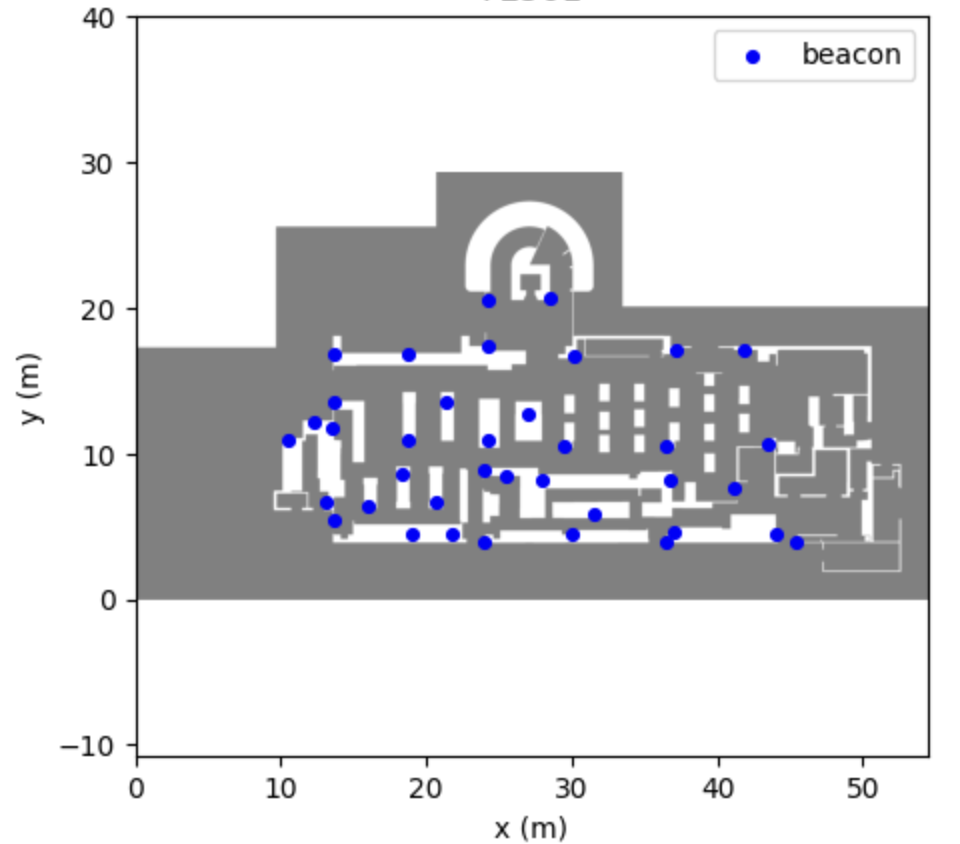
\includegraphics[width=\linewidth]{image/ble-beacon-position.jpg}
	\caption{BLEビーコンの基地局の位置情報}    \label{fig:ble-beacon-position}
\end{figure}

% TODO: 2.RSSIの値はデータの上位何%という風に決めた方がいいかも.
% 多くのビーコンを使用してなんとなくの全体像を把握するの重要なポイントな気がする
まず受信したRSSI値に対して閾値処理を行う.デフォルトではRSSIが-70dBmより
強い信号のみを使用する.この値は一般的なBLE信号の減衰特性を考慮して
設定されており,およそ3メートル程度の範囲内での受信信号に相当する.
この閾値は環境やユースケースに応じて調整可能であり,BLECorrectorの
初期化時にrssi\_thresholdパラメータとして指定できる.例えば
与えられるBLEスキャンデータの電波強度が強い割合が小さい場合は80dBm程度に緩和し,
逆に割合が多い場合は-65dbm程度に厳格化するといった調整が可能である.

この手法の特徴は建物の構造に依存せず,BLEビーコンが適切に配置されて
いれば任意の環境で適用可能な点にある.またRSSIの閾値の調整によって
補正の精度と信頼性のバランスを制御できる.ただしこの手法の
効果はBLEビーコンの配置密度や,環境内での電波伝搬特性に大きく
影響される点には注意が必要である.

次に選択された各BLE信号について,受信時刻に最も近い推定軌跡上の
ポイントを特定する.図\ref{fig:ble-merge}は,この対応付けの結果を
可視化したものである.軌跡上のポイントは時間経過に応じて色付けされており,
青色のポイントは対応するBLEビーコン基地局の位置を示している.

最後にこれらの対応点間の距離の総和が最小となるように軌跡全体の回転角度を
最適化する.受信時刻$t$における軌跡上の点と対応するビーコン基地局との
距離の総和$D(\theta)$を以下の式で表す:

\begin{equation}
D(\theta) = \sum_{t} \sqrt{(x_t(\theta) - b_x^t)^2 + (y_t(\theta) - b_y^t)^2}
\end{equation}

ここで$(x_t(\theta), y_t(\theta))$は角度$\theta$で回転させた軌跡上の
時刻$t$における座標,$(b_x^t, b_y^t)$は対応するBLEビーコン基地局の座標を表す.

\begin{equation}
\theta_{\mathrm{opt}} = \arg\min_{\theta \in [0, 2\pi]} D(\theta)
\end{equation}

この最適化問題は回転角度を$[0, 2\pi]$の範囲で探索することで解かれる.
この探索によりBLEビーコン基地局の位置と推定軌跡の位置関係が最も
整合する角度を見つけ最適な初期進行方向を決定できる.
% TODO 2.グリードサーチしている文章の説明がない気がする

\begin{figure}[H]
	\centering
	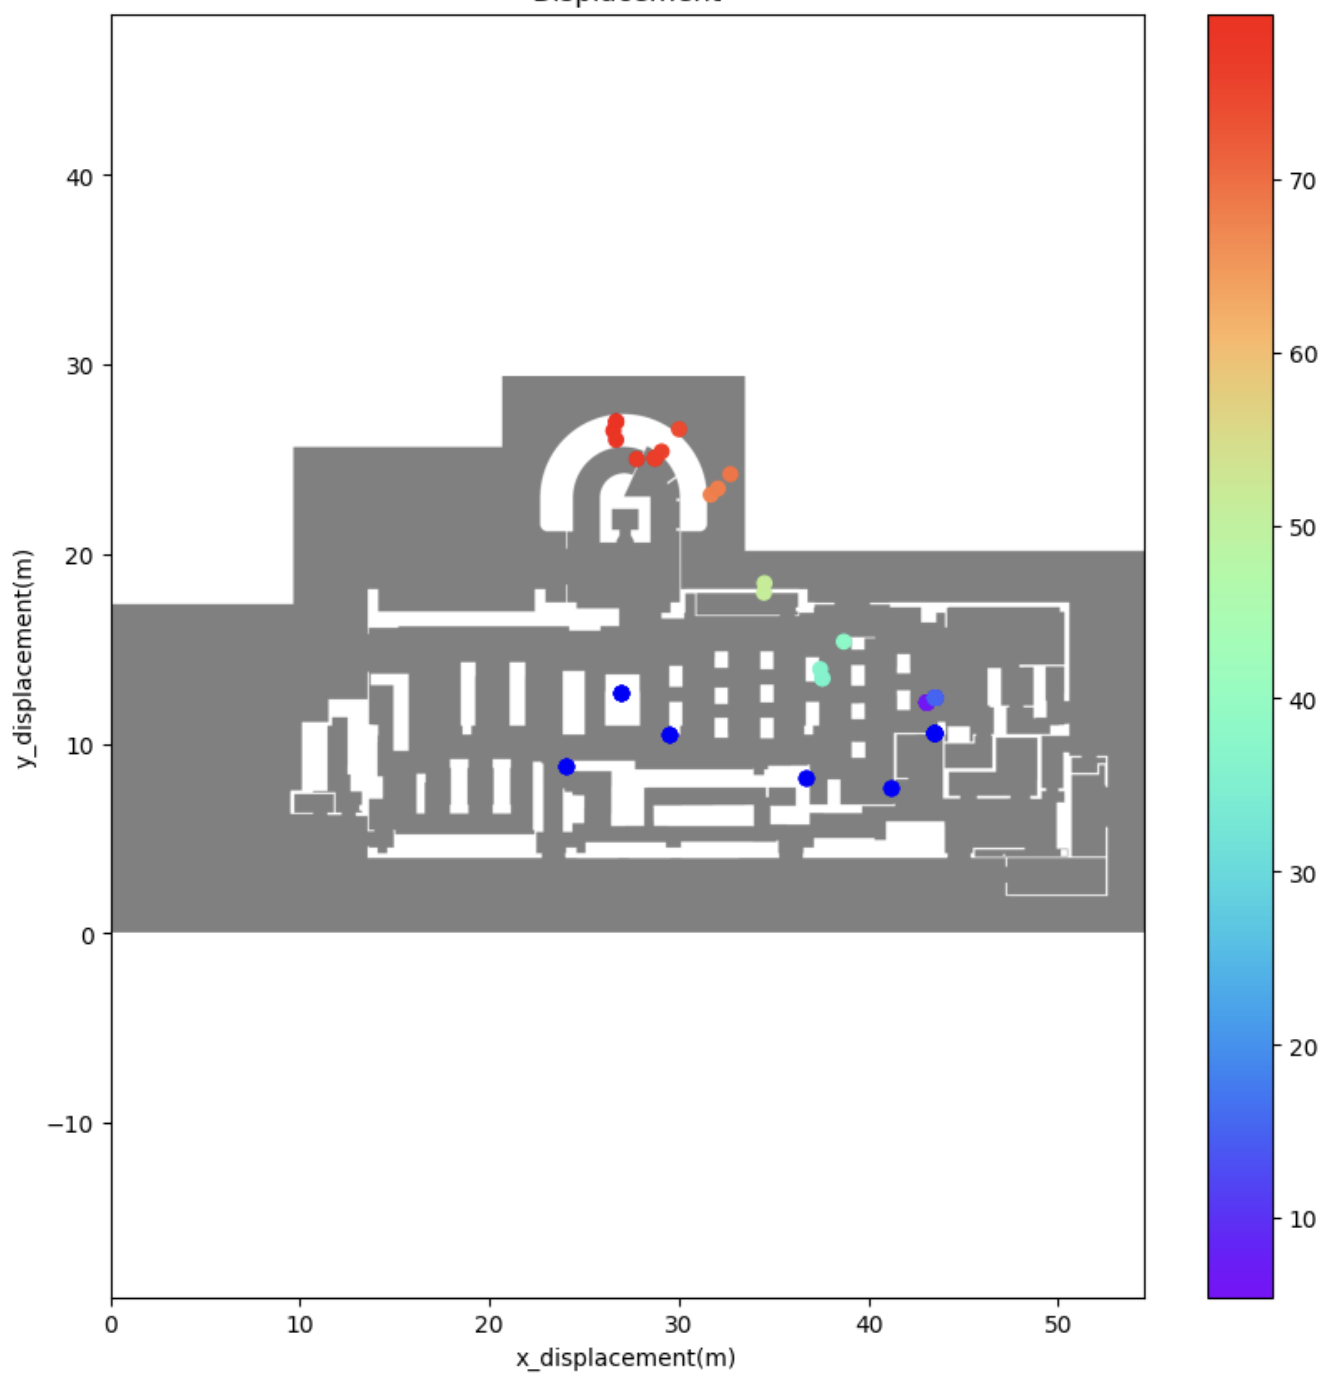
\includegraphics[width=\linewidth]{image/ble-merge.jpg}
	\caption{BLEビーコンの基地局の位置情報}    \label{fig:ble-merge}
\end{figure}


